% Created 2024-10-16 śro 21:35
% Intended LaTeX compiler: pdflatex
\documentclass[../main.tex]{subfiles}

% \usepackage[a4paper, margin=3cm]{geometry}
% \usepackage{amssymb} // not working

\usepackage[T1]{fontenc}
\usepackage[utf8]{inputenc}
\usepackage{graphicx}
\usepackage{longtable}
\usepackage{wrapfig}
\usepackage{rotating}
\usepackage[normalem]{ulem}
\usepackage{amsmath}
\usepackage{capt-of}
\usepackage{hyperref}
\usepackage{siunitx}
\usepackage{float}
\usepackage[polish]{babel}

\graphicspath{{../}}
\author{Wojciech Paderewski}
\date{\today}
\title{Serwery czasu}
\hypersetup{
 pdfauthor={Wojciech Paderewski},
 pdftitle={Serwery czasu},
 pdfkeywords={},
 pdfsubject={},
 pdflang={Polish}}

\begin{document}

Serwerem czasu nazywamy serwer komputerowy, pobierający czas z zewnętrznych źródeł i dystrybuuje go do innych urządzeń w sieci\cite{st:serwerczasu-book}.
Udostępniają bardzo precyzyjne dane czasowe, dokładność zależy od źródła czasu, z którego serwer korzysta. Serwer czasu może być używany jako lokalny lub internetowy.

Serwery wykorzystują rożne źródła zewnętrzne do synchronizacji czasu, takie jak:
\begin{itemize}
  \item zegary atomowe,
  \item odbioniki czasu GNSS (Global Navigation Satellite System),
  \item oscylatory rubinowe,
  \item oscylatory cezowe.
  \item zegary wodorowe
\end{itemize}

Są to zegary o bardzo dużej precyzji, rzędu nanosekund, co pozwala na synchronizację czasu w sieciach komputerowych, telekomunikacyjnych, itp.

\subsection{Protokoły synchronizacji czasu}
Serwery te Wykorzystują różne protokoły sieciowe do synchronizacji czasu, takie jak:
\begin{itemize}
  \item NTP (Network Time Protocol) - 
  Wysyła okresowo pakiety synchronizacji czasu do serwerów w sieci i odpowiednim dostosowywaniu zegarów lokalnych.
  Jest to najpopularniejszy protokół synchronizacji czasu w sieciach komputerowych, jest on wspierany przez większość systemów operacyjnych.
  \item PTP (Precision Time Protocol) - 
  jest bardziej precyzyjną alternatywą NTP i jest używany w systemach o wysokiej precyzji. Najczęściej stosowany w sieciach przemysłowych oraz przy badaniach naukowych. 
  Jest w stanie osiągnąć dokładność synchronizacji zegarów do poniżej mikrosekundy.
  \item Algorytm Berkeley - to algorytm synchronizacji czasu opracowany na Uniwersytecie Kalifornijskim w Berkeley. 
  Jego działanie polega na pomiarze szybkości dryfowania zegara między serwerami, często jest łączony z protokołem NTP.
  \item GPS -  wykorzystuje odbiorniki GPS do synchronizacji zegarów na różnych serwerach.
   Zapewnia bardzo dokładne sygnały czasu. Czas ten można wykorzystać do synchronizacji
  zegarów serwerów podłączonych do tego samego odbiornika GPS. 
\end{itemize}

\newpage

Każdy z tych protokołów ma swoje nastepujace wady i zalety:

\begin{itemize}
  \item NTP - Główną zaletą jest niezawodność i dokładność, co sprawia, że nadaje się do szerokiego zakresu zastosowań. 
  Jednak NTP nie jest tak dokładny jak PTP i może synchronizować zegary z dokładnością do kilku milisekund.
  W związku z tym, że jest to leciwy protokół, nie jest najbardziej bezpiecznym rozwiązaniem, 
  może być podatny na niektóre rodzaje ataków, takie jak ataki typu man-in-the-middle.
  Protokół istnieje już bardzo długo, więc dobrze znany i jest bardzo łatwy do obsługi.
  \item PTP - porównując do NTP, PTP jest bardziej precyzyjny i może synchronizować zegary z dokładnością do kilku mikrosekund.
  Jednak ma zdecydowanie większe wymagania sprzętowe(specjalistyczny sprzęt) i konfiguracyjne, co sprawia, że jest bardziej skomplikowany w użyciu.
  \item Algorytm Berkeley - możne być używać w połączeniu z NTP. 
  Jedną z głównych zalet tego algorytmu jest to, że może synchronizować zegary z dokładnością do kilku mikrosekund, dzięki czemu nadaje się do wielu zastosowań.
  Podobnie jak w PTP wymaga on specjalistycznego sprzętu, co sprawia, że jest bardziej skomplikowany w użyciu i droższy.
  \item GPS - najbardziej precyzyjny z wymienionych protokołów, może synchronizować zegary z dokładnością do kilku nanosekund.
  Jest jednak nie zalecany do zastosowań wewnątrz pomieszczeń, ze względu na konieczność widoczności satelitów GPS i wymaga odbiornika GPS.
\end{itemize} 

Z wyżej wymienionych protokołów, NTP jest najczęściej stosowany w sieciach komputerowych, dlatego też wydaje się być najlepszym wyborem do synchronizacji zegara nixie.
Alternatywnym rozwiązaniem mozę być wykorzystanie własnego serwera który by zwracał czas wykorzystując REST API, ale wymaga to posiadania własnego serwera i jest zależne od 
jego działania.

\subsection{Struktura serwerów w protokole NTP}
Synchronizacji NTP wykorzystuje uporządkowaną strukture gałęziowa STRATUM\cite{st:serwerczasu}. 
Zasada hierarchii wygląda nastepujaco: urządzenia warstwy STRATUM N mogą być serwerami czasu dla warstwy STRATUM N+1, ale nie na odwrót. 
Komputery STRATUM N mogą być również klientami urządzeń warstwy STRATUM N-1 itd.

Struktura ta ma na celu uporządkowanie i wprowadzenie hierarchii priorytetów urządzeń, zgodnie z ich rzeczywistym przeznaczeniem i funkcją. 
Aby nie nadmiernego skomplikowania systemu i związanych z tym opóźnień, ilość warstw została ograniczona do 16(STRATUM 0 - STRATUM 15).

Niektóre warstwy mają specjalne właściwości. Warstwa STRATUM 0 służy wyłącznie dla wzorców czasu, czyli zegarów atomowych, satelitarnych, itp. będących faktycznym źródłem czasu.
Połączenie ze źródłem nie jest sieciowe, a zazwyczaj odbywa się za pomocą specjalnych interfejsów sprzętowych.

STRATUM 1 oraz STRATUM 2 stanowią najwyższe warstwy NTP i powinny być wykorzystane w przypadku dużych serwerów
wysokiej jakości, superkomputerów lub sprzętowych serwerów czasu.
Pozostałe warstwy są przeznaczone dla urządzeń lokalnych, takich jak komputery, routery, itp.

Numer STRATUM mówi jak daleko od wzorca czasu znajduje się dany serwer. Im niższy numer, tym bliżej źródła czasu. 
W rozbudowanych sieciach poziom STRATUM nie ma znaczącego wpływu na jakość synchronizacji i precyzję uzyskiwanego czasu.

\begin{figure}[H]
  \centering
  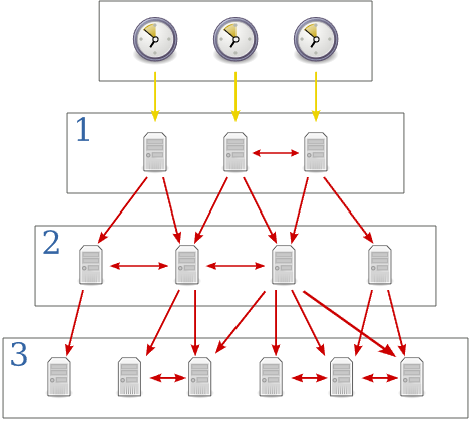
\includegraphics[width=0.5\textwidth]{serwers.png}
  \caption{Struktura serwerów czasu w protokole NTP\cite{st:serwerczasu-jpg}}
\end{figure}

W przypadku zegara nixie poziom STRATUM nie ma większego znaczenia, ponieważ zegar nie wymaga bardzo precyzyjnego czasu, chociaż oczywiście zależy,
jak precyzyjny czas będzie wyświetlany, ale w przypadku zegara na 6 cyfrach, różnica w czasie rzędu kilku milisekund nie będzie zauważalna.

\subsection{Zasada działania protokołu NTP}

NTP różni się od typowego protokołu komunikacyjnego. 
Nie transmituje on bowiem absolutnej wartości czasu, lecz przekazuje informacje o opoznieniach i korelacjach czasowych w regularnych odstępach czasu, jakie zachodzą w sieci TCP/IP. 
Protokół wyróżnia się dopiero przy stosowaniu wielu źródeł czasu jednocześnie, wykorzystuje od wtedy algorytm analizy statystycznej czasu oparty na metodzie DTS (Dynamic Time Scales).

NTP wykorzystuje pakiety UDP o długości 72 bajtów na porcie 123, które są okresowo wymieniane co ${2^\tau}$ sekund, gdzie ${\tau}$ wynosi od 4 (16s) do 17 (36h). 
Pozwala to klientom serwera, wyliczać opóźnienie względem idealnego czasu UTC.
Znając aktualne opóźnienie w odniesieniu do czasu UTC, klient NTP sam kalibruje swój zegar lokalny, która polega na płynnym przyspieszaniu lub spowalnianiu pracy lokalnego zegara programowego.
Przy różnicach czasu przekraczających 128ms, stosowana jest metoda step, która polega na skokowym przesunięciu zegara o określoną wartość.
Dzieki temu każdy z klientów, asymptotycznie zmierza do czasu pochodzącego z wzorcowego zegara czasu UTC.

\newpage

Sam pakiet NTP opisany jest w następujący sposób:

\begin{table}[H]
  \centering
  \begin{tabular}{|c|c|c|c|c|c|}
    \hline
    LI & VN & Mode & Stratum & Poll & Precision \\
    \hline
    \multicolumn{6}{|c|}{Root Delay} \\
    \hline
    \multicolumn{6}{|c|}{Root Dispersion} \\
    \hline
    \multicolumn{6}{|c|}{Reference Identifier} \\
    \hline
    \multicolumn{6}{|c|}{Reference Timestamp} \\
    \hline
    \multicolumn{6}{|c|}{Originate Timestamp} \\
    \hline
    \multicolumn{6}{|c|}{Receive Timestamp} \\
    \hline
    \multicolumn{6}{|c|}{Transmit Timestamp} \\
    \hline
    \multicolumn{6}{|c|}{Authenticator} \\
    \hline
  \end{tabular}
  \caption{NTP – format komunikatu}

\end{table}

\begin{itemize}
  \item LI – wskaźnik sekund przestępnych
  \item VN – (Version Number) numer wersji protokołu
  \item   Mode – tryb pracy
  \item Stratum – warstwa, w której funkcjonuje komputer będący nadawcą komunikatu
  \item Poll interval – okres pomiędzy kolejnymi aktualizacjami czasu
  \item Precision – określenie dokładności zegara komputera wysyłającego dany komunikat
  \item Root Delay – opóźnienie pomiędzy nadawcą a serwerem warstwy 1
  \item Root Dispersion – maksymalny błąd pomiędzy zegarem lokalnym a serwera warstwy 1
  \item Reference Identifier – identyfikator źródła czasu, względem którego następuje synchronizacja
  \item Reference Timestamp – pole zawierające pomocnicze informacje o czasie poprzedniej synchronizacji
  \item Originate Timestamp – pole zawierające czas wysłania żądania przez klienta
  \item Receive Timestamp – czas odebrania komunikatu od klienta
  \item Transmit Timestamp – czas wysłania odpowiedzi do klienta
  \item Authenticator – informacje uwierzytelniające zarówno klienta, jak i serwer czasu
  \item Root Dispersion – maksymalny błąd pomiędzy zegarem lokalnym a serwera warstwy 1
  \item Reference Identifier – identyfikator źródła czasu, względem którego następuje synchronizacja
  \item Reference Timestamp – pole zawierające pomocnicze informacje o czasie poprzedniej synchronizacji
  \item Originate Timestamp – pole zawierające czas wysłania żądania przez klienta
  \item Receive Timestamp – czas odebrania komunikatu od klienta
  \item Transmit Timestamp – czas wysłania odpowiedzi do klienta
  \item Authenticator – informacje uwierzytelniające zarówno klienta, jak i serwer czasu
\end{itemize}

\end{document}
